% Chapter Template

\chapter{The Birkhoff Polytope} % Main chapter title

\label{ChapterX} % Change X to a consecutive number; for referencing this chapter elsewhere, use \ref{ChapterX}



%----------------------------------------------------------------------------------------
%	SECTION 1
%----------------------------------------------------------------------------------------
In this Chapter I am going to describe about Birkhoff polytope $B_n$ which is sometimes considered to be one of the most important polytopes in many sphere. Before that I will define some basic types.
\section{Hypermatrix}

A generalisation of matrix to an $n_1 \times n_1 \times ...$ array of numbers. \newline
Example: 3-dimensional hypermatrix(cube). It is a $2 \times 2 \times 2$ matrix over $\mathbb{R}$.


\begin{figure}[h]
\centering
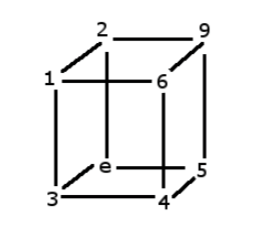
\includegraphics{Figures/hypercube.png}
\decoRule
\caption[hypercube]{3-dimensional hypermatrix(cube).}
\label{fig:hypercube}
\end{figure}

\section{Doubly-Stochastic Matrix}

Doubly Stochastic Matrix is a square matrix of non-negative real numbers, each of whose rows and columns sum to 1. If rows and columns of some matrices sum to n, it can also be considered as doubly stochastic matrix because we can just device all the entries by n, which results to true Doubly Stochastic.\\


Examples:

\[
  \begin{bmatrix}
    0 & 1 & 0 \\
    1 & 0 & 0 \\
    0 & 0 & 1 \\
  \end{bmatrix}
  ,
    \begin{bmatrix}
     1/6 & 5/6 & 0 & 0 \\
     0 & 0 & 1 & 0 \\
     0 & 1/6 & 0 & 5/6 \\
     5/6 & 0 & 0 & 1/6
    \end{bmatrix}
  ,
    \begin{bmatrix}
     \frac{1}{2} & \frac{1}{2} \\
     \frac{1}{2} & \frac{1}{2}
    \end{bmatrix}
\]

\section{Permutation Matrix}

A matrix obtained by permuting the rows of an $n\times n$ identity matrix according to some permutation of the numbers 1 to n. So the number of $n\times n$ permutation matrics is $n!$.\\

The permutation matrics of order 3 are:
\[
  \begin{bmatrix}
    1 & 0 & 0 \\
    0 & 1 & 0 \\
    0 & 0 & 1 \\
  \end{bmatrix}
  ,
    \begin{bmatrix}
     1 & 0 & 0 \\
     0 & 0 & 1 \\
     0 & 1 & 0 \\
    \end{bmatrix}
  ,
    \begin{bmatrix}
     0 & 0 & 1 \\
     1 & 0 & 0 \\
     0 & 1 & 0 \\
    \end{bmatrix}
    ,
    \begin{bmatrix}
     0 & 1 & 0 \\
     1 & 0 & 0 \\
     0 & 0 & 1 \\
    \end{bmatrix}
    ,
    \begin{bmatrix}
     0 & 1 & 0 \\
     0 & 0 & 1 \\
     1 & 0 & 0 \\
    \end{bmatrix}
    ,
    \begin{bmatrix}
     0 & 0 & 1 \\
     0 & 1 & 0 \\
     1 & 0 & 0 \\
    \end{bmatrix}
\]


\section{Polytopes}

In elementary geometry, a polytope is a geometric object with flat sides, and may exist in any general number of dimensions n as an n-dimensional polytope or n-polytope. For example a two-dimensional polygon is a 2-polytope and a three-dimensional polyhedron is a 3-polytope

Mathematically, A polytope $P\subseteq \mathbb{R}^d$ is the convex hull $P=conv(v_1,...,v_k)$ of a finite set of points $v_1,...,v_k \in \mathbb{R}^d$ . Dually any polytope can be written as the bounded intersection of a finite number of affine half-spaces in the form $P = \{ x\mid Ax \leq b \}$

\subsection{Elements of polytope}
A proper face of $F$ of a polytope $P$ is the intersection of $P$ with and affine hyperplane $H$ such that $P$ is completely contained in one of the closed half spaces defined by $H$. The empty set and the polytope P a face of $P$. Any face $F$ is itself  polytope. The dimension of a polytope $P \subseteq \mathbb{R}^d$ is the dimension of the minimum affine space containin it. It is full dimensional if its dimension is d.

0-dimensional faces of $P$ are called $vertices$, 1-dimensional faces are edges. Proper faces of maximal dimensional are called facets. $P$ is the convex hull of its vertices, and the vertices of any face are subset of the vertices of $P$. Thus, a polytope has only a finite number of faces. Let $f_i$ be the number of $i$-dimensional faces of $P,0 \leq i \leq dim P-1$. The $f$-vector of a d-dimensional polytope P is the non-negative integral vector $f(P) = (f_0,...,f_(d-1)$.

The face lettice or combinatorial type $\mathcal{L}(P)$ of a polytope P is the partially ordered set of all faces of P (including the empty face and P itself). This defines Eulerian lattice. Figure shows 2.1 this lattice.


It contains all combinatorial information of the polytope. Two polytopes P,$P'$ are combinatorially isomorphic or have the same combinatorial type if their face lattices are isomorphic as posets.

An r-dimensional simplex (or r-simplex) is the convex hull of r+1 affinely independent points in $\mathbb{R}^d$. A polytope is called simplicial if all facets are simplices. It is simple if the dual is simplicial. Equally, a d-dimensilanl polytope P is simple if each vertex is incident to precisely d edges. The d-dimensional 0/1-cube $C^d$ is the convexhull of all d-dimensinal 0/1-vectors. This is a simple d-polytope with $2^d$ vertices and 2d facets. More generally we denote by a d-cube any d-dimensional polytope that is combinatorially isomorphic to the 0/1-cube (it need not be full dimensional).

\subsection{Properties of Polytope}
Let $P_1 \subset \mathbb{R}^{d_1}$ and $P_2 \subset \mathbb{R}^{d_2}$ be two (geometrically realized) polytopes with vertex sets $V(P_1)=\{ v_1,...,v_k$ and $V(P_2)=\{ w_1,...,w_l \}$. With $0^{(d)}$ we denote he d-dimensional zero vector.

The (geometric) product of $P_1$ and $P_2$ is the polytope

\begin{equation}
P_1 \times P_2 = conv( (v_i,w_i)\in \mathbb{R}^{d_1+d_2}\mid 1\leq i \leq k, i \leq j \leq l)
\label{eqn:Einstein}
\end{equation}

This is the same as the set of all points $(v,w)$ for $v \in P_1$ and $w \in P_2$. The (geometric) join of $P_1$ and $P_2$ is the polytope

\begin{equation}
P_1 \star P_2 := conv(P_1 \times \{ 0^{d_2} \} \times \{ 0 \} \cup \{ 0^{d_1} \} \times P_2 \times \{ 1 \} ) \subseteq \mathbb{R}^{d_1+d_2+1}
\label{eqn:Einstein}
\end{equation}

More generally we say that a polytope P is a product or join of two polytopes $P_1$ and $P_2$, if P is combinatorially isomorphic to the geometric prouct or geometric join of some realisations of the face lattices $P_1$, or $P_2$.

If $F$ is face of a polytope  $P = \{ x \mid Ax \leq b \} \subseteq \mathbb{R}^d$  and $ \langle c,x \rangle \leq d $ a linear funtional defining F, then the $wedge wedge_F(P)$ of P over F is defined to be the polytope.
 
\begin{equation}
wedge_F(P) = \{ (x,x_0) \in \mathbb{R}^{d+1} \mid Ax\leq b, 0\leq x_0 \leq d- \langle c,x \rangle\}
\label{eqn:Einstein}
\end{equation}

Again, we say more generally that P is wedge of a polytope  Q over some face F of Q if P is combinatorially equivalently to $wedge_F(Q)$



%----------------------------------------------------------------------------------------
%	SECTION 2
%----------------------------------------------------------------------------------------

\section{Birkhoff Polytope}

Birkhoff polytope $B_n$ is sometimes considered to be one of the most important polytopes in many sphere. Birkhoff polytope is also called assignment polytope, the polytope of doubly stochastic matrices, or the perfect matching polytope of complete bipartite graph $K_(n,n)$ ,transportation polytope. It surprisingly appears in various branches of mathematics from geometry to enumerative combinatorics to optimisation theory to Statistics.

The Birkhoff polytope $B_n$ is the convex hull of all $(n\times n)$ permutation metrices, i.e.matrices which consists precisely one 1 in every row and column, and zeros at all places. Equivalently, $B_n$ is the set of all non-negative $(n \times n)$-metrices, whose rows and columns all sum to 1, or the perfect matching polytope of the complete bipartite graph $K_(n,n)$. The Birkhoff polytope $B_n$ has dimension $(n-1)^2$ with $n!$ vertices and $n_2$ facets. The Birkhoff-von Neumann Theoram illustrated, $B_n$ can be understood as the intersection of the positive orthant with a family of of hyperplanes.

Birkhoff polytopes are widely studied as a class of polytopes in the area of optimisation, statistics, enumerative combinatorics or representation theory. Despite, Combinatorial and Geometrical structure of Birkhoff polytope and its algorithmic treatment are still open to disover.

A Birkhoff polytope $B_n$ is a polytope defined by the following equations and in-equalities:
\begin{equation}
a_{i,j} \geqslant 0, \sum_{i=1}^{n} a_{i,j} = 1, \sum_{j=1}^{n} a_{i,j}=1 \text{ for all } 1\leqslant i,j\leqslant n.
\label{eqn:Birkhoff_definition}
\end{equation}	

$(a_{i,j}$ can be thought of as  $n\times n$ doubly stochastic matrices. It can be realise that $B_n$ has dimension $(n-1)^2$ as values of $a_{i,j},1\leqslant i,j\leqslant n$ determine the rest. Different way helps to realise that vertices of $P_n$ are permutation matrices.

\section{Properties of $\B_n$}

\subsection{Vetices}
The Birkhoff polytope has $n!$ vertices, one for each permutation on $n$ items. 




 Let $S_n$ be the group of permutations on $n$ elements. To any element $\sigma \in S_n$ we can associate a 0/1-matrix $M( \sigma ) \in \mathbb{R}^{n \times n}$ that has a 1 at position (i,j) if and only if $\sigma(i)=j$. The n-th Birkhoff polytope is:
\begin{equation}
\mathbb{B} = conv(M( \sigma ) \mid \sigma \in S_n ) \subseteq \mathbb{R}^{n \times n}
\label{eqn:Einstein}
\end{equation}	

The Birkhoff-von Neumann Theorem shows that $\mathbb{B}_n$ can equally be characterized as the set of all non-negative $(n \times n)$ -matrices whose rows and columns all sum to 1. Equivalently, the facets of $\mathbb{B}_n$ are precisely defined by the inequalities $x_{ij} \geq 0 for 1 \leq i, j \leq n$. It has dimension $(n-1)^2$ with $n^2$ facets and $n!$ vertices.



%-----------------------------------
%	SUBSECTION 1
%-----------------------------------
\subsection{Subsection 1}

Nunc posuere quam at lectus tristique eu ultrices augue venenatis. Vestibulum ante ipsum primis in faucibus orci luctus et ultrices posuere cubilia Curae; Aliquam erat volutpat. Vivamus sodales tortor eget quam adipiscing in vulputate ante ullamcorper. Sed eros ante, lacinia et sollicitudin et, aliquam sit amet augue. In hac habitasse platea dictumst.


%-----------------------------------
%	SUBSECTION 2
%-----------------------------------

\subsection{Subsection 2}
Morbi rutrum odio eget arcu adipiscing sodales. Aenean et purus a est pulvinar pellentesque. Cras in elit neque, quis varius elit. Phasellus fringilla, nibh eu tempus venenatis, dolor elit posuere quam, quis adipiscing urna leo nec orci. Sed nec nulla auctor odio aliquet consequat. Ut nec nulla in ante ullamcorper aliquam at sed dolor. Phasellus fermentum magna in augue gravida cursus. Cras sed pretium lorem. Pellentesque eget ornare odio. Proin accumsan, massa viverra cursus pharetra, ipsum nisi lobortis velit, a malesuada dolor lorem eu neque.

%----------------------------------------------------------------------------------------
%	SECTION 3
%----------------------------------------------------------------------------------------

\section{Main Section 2}

Sed ullamcorper quam eu nisl interdum at interdum enim egestas. Aliquam placerat justo sed lectus lobortis ut porta nisl porttitor. Vestibulum mi dolor, lacinia molestie gravida at, tempus vitae ligula. Donec eget quam sapien, in viverra eros. Donec pellentesque justo a massa fringilla non vestibulum metus vestibulum. Vestibulum in orci quis felis tempor lacinia. Vivamus ornare ultrices facilisis. Ut hendrerit volutpat vulputate. Morbi condimentum venenatis augue, id porta ipsum vulputate in. Curabitur luctus tempus justo. Vestibulum risus lectus, adipiscing nec condimentum quis, condimentum nec nisl. Aliquam dictum sagittis velit sed iaculis. Morbi tristique augue sit amet nulla pulvinar id facilisis ligula mollis. Nam elit libero, tincidunt ut aliquam at, molestie in quam. Aenean rhoncus vehicula hendrerit.